\documentclass{standalone}
\usepackage{graphicx}	
\usepackage{amssymb, amsmath}
\usepackage{color}

\usepackage{tikz}
\usetikzlibrary{calc, arrows.meta}
\usepackage{pgfmath}

\definecolor{light}{RGB}{220, 188, 188}
\definecolor{mid}{RGB}{185, 124, 124}
\definecolor{dark}{RGB}{143, 39, 39}
\definecolor{highlight}{RGB}{180, 31, 180}
\definecolor{gray10}{gray}{0.1}
\definecolor{gray20}{gray}{0.2}
\definecolor{gray30}{gray}{0.3}
\definecolor{gray40}{gray}{0.4}
\definecolor{gray60}{gray}{0.6}
\definecolor{gray70}{gray}{0.7}
\definecolor{gray80}{gray}{0.8}
\definecolor{gray90}{gray}{0.9}
\definecolor{gray95}{gray}{0.95}

\newcommand*{\offset}{0.025}

\begin{document}

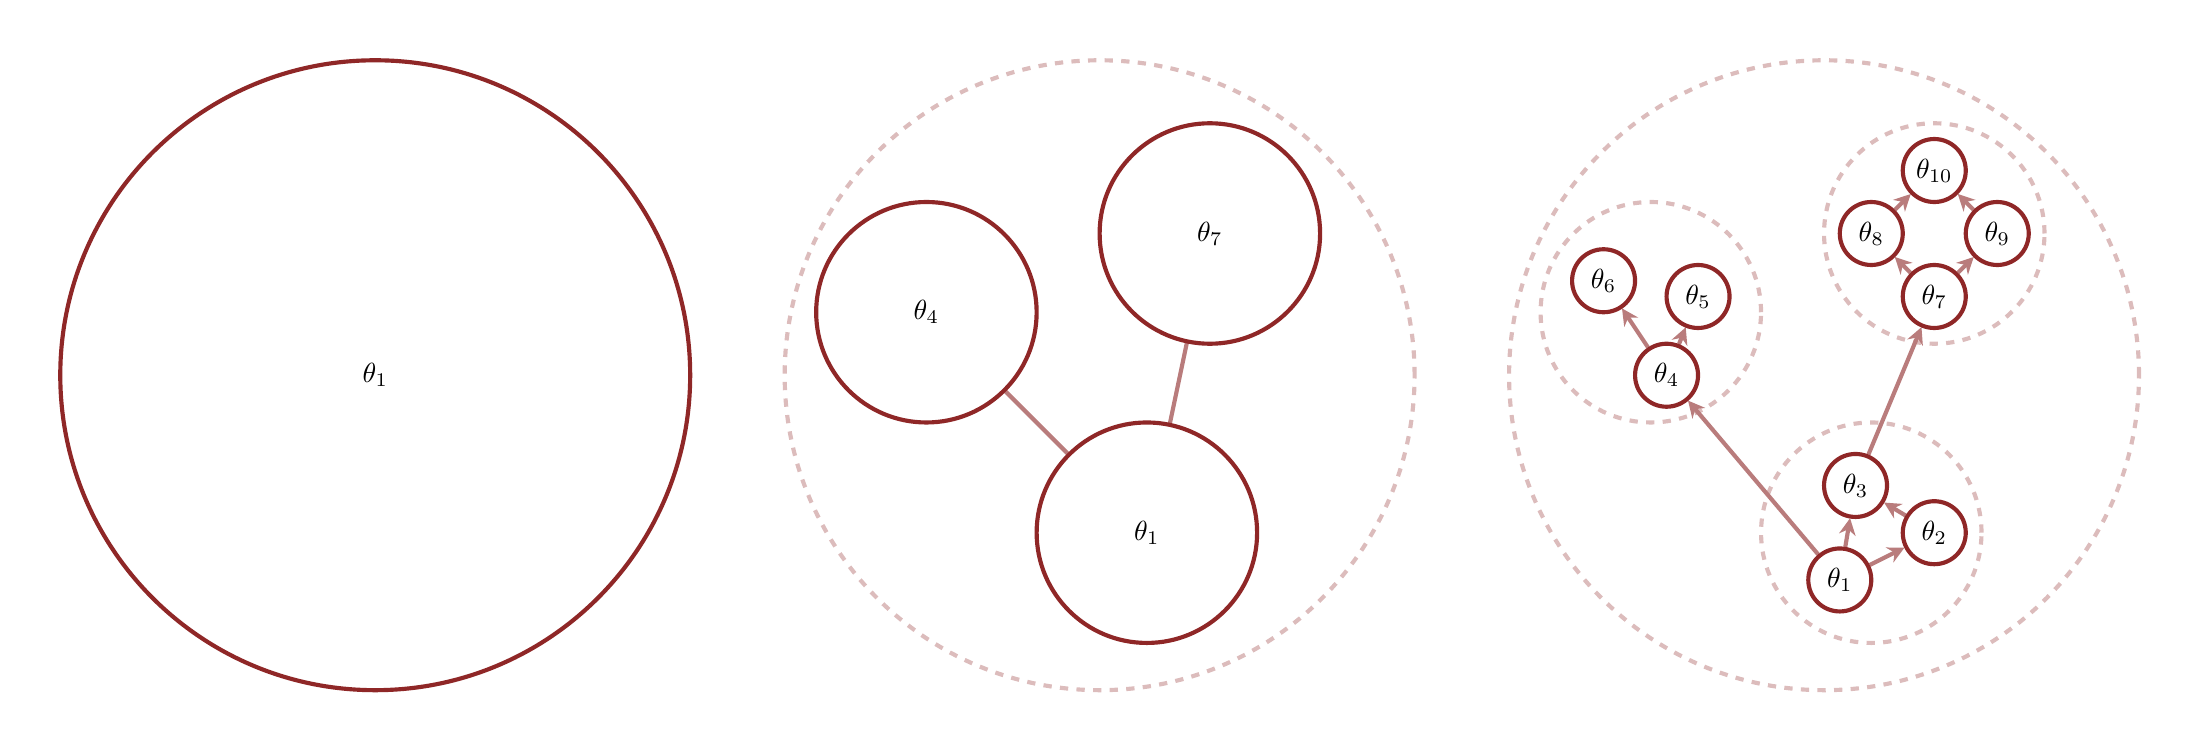
\begin{tikzpicture}[scale=0.2, thick]

  \pgfmathsetmacro{\r}{2}
    
  \begin{scope}[shift={(0, 0)}]
    \draw[white] (-21, -2) rectangle (23, 42);

    \coordinate (A) at (1, 20);
    
    \filldraw[fill=white, draw=dark, line width=1.5] (A) circle (20)
    node[color=black] { $\theta_{1}$ };
    
  \end{scope}
  
  \begin{scope}[shift={(46, 0)}]
    \draw[white] (-21, -2) rectangle (23, 42);

    \coordinate (A) at (4, 10);
    \coordinate (B) at (-10, 24);
    \coordinate (C) at (8, 29);
    
    \draw[light, dashed, line width=1.5] (1, 20) circle (20);
  
    \foreach \B/\E in {A/B, A/C} {
      \draw[-{Stealth[length=6pt, width=6pt]}, shorten <=12.1, shorten >=12, color=mid, line width=1.5] (\B) -- (\E);
    }

    \filldraw[fill=white, draw=dark, line width=1.5] (A) circle (7)
    node[color=black] { $\theta_{1}$ };
    
    \filldraw[fill=white, draw=dark, line width=1.5] (B) circle (7)
    node[color=black] { $\theta_{4}$ };
    
    \filldraw[fill=white, draw=dark, line width=1.5] (C) circle (7) 
    node[color=black] { $\theta_{7}$ };
    
  \end{scope}
  
  \begin{scope}[shift={(92, 0)}]
    \draw[white] (-21, -2) rectangle (23, 42);
  
    \coordinate (A) at (2, 7);
    \coordinate (B) at (8, 10);
    \coordinate (C) at (3, 13);

    \coordinate (D) at (-9, 20);
    \coordinate (E) at (-7, 25);
    \coordinate (F) at (-13, 26);
    
    \coordinate (G) at (8, 25);
    \coordinate (H) at (4, 29);
    \coordinate (I) at (12, 29);
    \coordinate (J) at (8, 33);
    
    \draw[light, dashed, line width=1.5] (1, 20) circle (20);
    
    \draw[light, dashed, line width=1.5] (4, 10) circle (7);
    \draw[light, dashed, line width=1.5] (-10, 24) circle (7);
    \draw[light, dashed, line width=1.5] (8, 29) circle (7);

    \foreach \B/\E in {A/B, A/C, B/C, A/D, D/E, D/F, C/G, G/H, G/I, H/J, I/J} {
      \draw[-{Stealth[length=6pt, width=6pt]}, shorten <=12.1, shorten >=12, color=mid, line width=1.5] (\B) -- (\E);
    }

    \filldraw[fill=white, draw=dark, line width=1.5] (A) circle (\r)
    node[color=black] { $\theta_{1}$ };
    
    \filldraw[fill=white, draw=dark, line width=1.5] (B) circle (\r)
    node[color=black] { $\theta_{2}$ };
    
    \filldraw[fill=white, draw=dark, line width=1.5] (C) circle (\r) 
    node[color=black] { $\theta_{3}$ };
    
    \filldraw[fill=white, draw=dark, line width=1.5] (D) circle (\r)
    node[color=black] { $\theta_{4}$ };
      
    \filldraw[fill=white, draw=dark, line width=1.5] (E) circle (\r)
    node[color=black] { $\theta_{5}$ };

    \filldraw[fill=white, draw=dark, line width=1.5] (F) circle (\r)
    node[color=black] { $\theta_{6}$ };

    \filldraw[fill=white, draw=dark, line width=1.5] (G) circle (\r)
    node[color=black] { $\theta_{7}$ };
    
    \filldraw[fill=white, draw=dark, line width=1.5] (H) circle (\r)
    node[color=black] { $\theta_{8}$ };
    
    \filldraw[fill=white, draw=dark, line width=1.5] (I) circle (\r)
    node[color=black] { $\theta_{9}$ };
    
    \filldraw[fill=white, draw=dark, line width=1.5] (J) circle (\r)
    node[color=black] { $\theta_{10}$ };
    
  \end{scope}

\end{tikzpicture}

\end{document}  